\pdfoutput=1 % only if pdf/png/jpg images are used
\documentclass{JINST}

\usepackage{amsmath,amssymb}
\usepackage[numbers,sort]{natbib}
%\hypersetup{colorlinks, citecolor=blue, linkcolor=blue, filecolor=blue, urlcolor=red}

\title{PETALO, a new concept for a Positron Emission TOF apparatus using Liquid xenon}

\author{J. J. Gomez-Cadenas$^a$,J. M. Benlloch-Rodriguez$^a$, P. Ferrario$^a$\thanks{Corresponding author.}, 
F. Monrabal$^a$, J.F. Toledo$^b$

\llap{$^a$}IFIC\\
\llap{$^b$}UPV\\
\llap{$^b$}Instituto de F\'isica Corpuscular (IFIC), CSIC \& Universitat de Val\`encia,\\ 
Calle Catedr\'atico Jos\'e Beltr\'an, 2, 46980 Paterna, Valencia, Spain\\

E-mail: \email{gomez@mail.cern.ch}}

\bibliographystyle{unsrtnat}
\input{commands}

\abstract{We describe a new Positron Emission Tof Apparatus using Liquid xenOn (PETALO). The detector is based in the {\em  Liquid Xenon Scintillating Cell (LXSC)}.The cell is a box of filled with liquid xenon and immersed in a cryostat. The cell transverse size (relative to the incoming beam) is optimised to minimise pileup and its longitudinal size is optimised so that most of the incoming 511 keV photons (80\%) interact in the volume. The best performance is obtained when all the box faces are instrumented with large (6 mm) silicon fotomultipliers (SiPMs) densely packed and coated with a wavelength shifter, Tetraphenyl butiadene (TPB). We denote this configuration as LXSC6. The most economical configuration is obtained instrumenting only the entry and exit faces (relative to the incoming gammas direction). The faces non instrumented are covered by reflecting teflon coated with TPB. We call this configuration LXSC2. Our Monte Carlo studies indicate that an excellent performance can be obtained even with the most sparse configurations (LXSC2).The LXSC constitutes the core of a high-sensitivity, nuclear magnetic resonance compatible, PET device, with enhanced Time Of Flight (TOF) sensitivity.}

\keywords{PET; TOF; Liquid Xenon; Nuclear Magnetic Resonance; energy resolution; high sensitivity.}


\begin{document}

\section{Introduction}

%\section{Positron Electron Tomography}
\label{sec.intro}

A PET (Positron-Electron Tomography) is a functional scan ---it does not show anatomic features--- whose main application is tumor diagnosis. It is based in the used of positron emitters radio-pharmaceuticals such as the fluorodeoxyglucose (FDG). Such radiotracers 
are injected into the patient prior to the scan. The emitted positrons slow down in the surrounding patient's tissue, annihilating with atomic electrons to give two back-to-back 511 keV annihilation photons.  By detecting the two photons in coincidence and the coordinates of their interaction points in a detector, it is possible to define a line of response (LOR) along which the positron emitting source is located in the patient. A set of such intersecting lines allows 3D reconstruction of the source. 

The main requirements for a PET detector are: (a) high photon detection efficiency ($\sim$ 80\% for each 511 keV gamma), (b) position resolution of a few millimeters, (c) time resolution to reduce the rate of false coincidences, (d) good energy resolution (20\% FWHM is typical in many commercial devices) to discriminate photons scattered in the patient and (e) a high count rate capability ($\sim10^6$~ s$^{-1}$ per cm$^2$~ of detecting surface). In addition, a PET system must have an angular acceptance as large as possible, which in turn requires a large axial (along the patient's body) coverage. However, due to the high cost of this devices, the axial size  of a PET is typically limited to 15-25 cm. 

Today's PET scanners use Solid Scintillating Detectors (SSDs) such as Sodium Iodine (NaI), Bismuth Germanate (BGO) or Lutetium (ytrium) oxyorthosilicate (LSO/LYSO), readout by light sensitive detectors. The standard has shifted from the use of NaI crystals, to the use of LSO/LYSO devices. Until recently, the SSDs were readout with photomultipliers (PMTs), but  Silicon Photomultipliers (SiPMs) are emerging in the last few years a a major alternative. Unlike PMTs, SiPMs can be used in the presence of a strong magnetic field, therefore opening the possibility to build Magnetic Resonance Imaging (MRI) compatible PET devices. 

The physical properties that define a detector suitable for a PET scanner are: 
\begin{enumerate}
\item {\bf Attenuation length ($\lambda$)}, which sets the scale of the length (across the photon line of flight) that the detector has to have in order to stop most of the incoming radiation.
\item {\bf Density ($\rho$)}, which is related with the total size and weight of the detector.
\item {\bf Photon yield per keV ($Y$)}, which must be as high as possible to record large signals. 
\item {\bf Energy resolution at 511 keV ($\sigma_E$)}, which must be as good as possible. 
\item {\bf Transverse spatial resolution ($\sigma_T$)} (relative to the photon line of flight), which in turn depends on the photon yield and the granularity of the readout sensors.
\item {\bf Longitudinal spatial resolution ($\sigma_L$)}, important to minimise the so-called parallax error.  $\sigma_L$~  tends to be poor for the SSDs, which do not measure the longitudinal coordinate (thus $\sigma_L \sim L/\sqrt{12}$, where $L$~is the detector length). 
\item {\bf Scintillation decay time ($t_s$)}, which must be as fast a possible, to maximise the number of events acquired per unit time and to minimise the window used to correlate events in different crystals. In addition, if the system has very good time resolution (in the range of few hundred picoseconds) time-of-flight measurements (TOF) are possible.  
\end{enumerate}


\paragraph{Liquid Xenon as detection material:}

Xenon is a noble gas. It responds to ionising radiation providing both ionisation and scintillation signals. The ionisation signal is due to atomic electrons ejected from the xenon atoms by the incoming radiation, which take a long time to recombine due to the noble-gas nature of xenon (and therefore can be drifted to a collection electrode, if so desired). The scintillation signal is due to the de-excitation of xenon atoms forming dimers which decay after 2.2 ns (dominant single mode) or 27 ns (triplet mode) emitting ultraviolet light (VUV) of 178 nm wavelength.

In its liquid phase (at a temperature of 165 K and 1 bar of pressure) LXe has a reasonable high density and an acceptable attenuation length, which makes it suitable for PET applications. Its advantage with respect to SSD are: a) its very high yield, which in turn can translate in excellent energy and transverse spatial resolution; b) Its ability to provide a 3D measurement of the interaction point, thus a high-resolution measurement of the longitudinal coordinate, minimising parallax errors; c) its capability to identify Compton events depositing all its energy in the detector as separate-site interaction, due to the relatively large interaction length in xenon;  d) its very fast scintillation decay time, which makes it suitable as a TOF-PET;  and e) its relatively low cost (e.g, about 10\% of the cost of LSO per unit detector).  Table \ref{table.SDPP} shows the physical properties of common PET SD compared with that of liquid xenon (LXe). 


\begin{table}[htdp!]
\caption{Physical properties of common PET SSD and of LXe}
\begin{center}
\begin{tabular}{|l||c|c|c|c|}
\hline
& NaI & BGO & LSO & LXe\\
\hline
Effective $Z$ & 50 & 74 & 66 & 54 \\
$\rho$~(g/cm$^3$) & 3.7 & 7.1 & 7.4 &  3 \\
$\lambda$ ~ at 511 keV (mm) & 28 & 11 & 12 & 36 \\
$Y$~per keV & 38 & 6 & 29 & {\bf 72} \\
%RLO & 100 & 15 & 75 & {\bf 190} \\
$t_s$~(ns) & 230 & 300 & 40 & {\bf 2.2} \\
\hline
\end{tabular}
\end{center}
\label{table.SDPP}
\end{table}%

The first idea of using a LXeTPC for PET was proposed in 1993 by Chepel\footnote{{\em Chepel, V. Y. et al}, in Proceedings on The International
Workshop on Technique and Application of Xenon Detectors (Xenon 01), University of Tokyo, December 2001.}. The proposed detector was a LXe multi-wire detector consisting of six ionisation cells, each formed by two parallel cathode plates with a multi-wire anode in the middle. 
Subsequent R\&D is documented in \footnote{{\em Chepel, V. Y. et al.}, 1995, Nucl. Instrum. Methods A
367, 58; {\em Chepel, V. Y. et al.}, 1994, Nucl. Instrum. Methods
A349, 500; {\em Chepel, V. Y. et al.}, 1997, Nucl. Instrum. Methods A392, 427; {\em Chepel, V. Y. et al., 1999, IEEE Trans NS-46, 1038}; {\em Crespo, P. et al.}, 1998, IEEE Trans. NS-45, 56; {\em Crespo, P. et al.}, 2000, IEEE Trans, NS-47, 2119; {\em Lopes, M. I. et al.}, 1995, IEEE Trans. NS-42, 2298.; {\em Thers D.}, ``A Positron Emission Tomograph (PET)
based on a liquid Xenon Time Projection Chamber and Microstructure Devices for Compton tracking'', in Workshop on LXe-PET Camera, Subatech, Nantes, France, October 2003; }. {\bf All those devices were based in the exploration of the ionisation signal in LXe}. {\em However, the measurement of such signals introduces a severe constrain to the technique, given the slow drift time of electrons in LXe} (typically of the order of 2 mm/$\mu$s, for a drifting field of 
1 KV/cm). Since $\lambda = 3$.6~cm the practical length of a LXe cell (along the photon line of flight) must be of 5 cm to contain 80 \% of the photons. This, in turn, implies drifting times of 25 $\mu$s, which limits the interaction rate that can be recorded by the cell to  
$\sim10^5 s^{-1}$, and therefore imposes a low-rate PET with a limited range of applications. 

On the other hand, the possibility of building a LXe PET (with TOF capabilities) based on the excellent properties of LXe as scintillator, was first suggested by Lavoie in 1976\footnote{{\em Lavoie L.}, 1976, Medical Physics 3, No. 5, 283.}, and the study of this type of PET was carried out by the Waseda group \footnote{{\em Doke T., J. Kikuchi, and F. Nishikido}, 2006, 
Nucl. Instrum. Methods A 569, 863;  {\em Nishikido, F. et al.}, 2005, Jpn J. Appl. Phys. 44, 5193; {\em Nishikido, F. et al.}, 2004, Jpn J. Appl. Phys. 43, 779.}. The Waseda prototype was based in LXe cells read out by VUV-sensitive PMTs. In those cells one of the sides was left instrumented. The relatively poor performance of the system can be attributed in part to the use of PMTs and in part to the partial lack of instrumentation which affected both the energy and the time resolution. The PMTs, although sensitive to the VUV light emitted by xenon had low quantum efficiencies (in the range 5-25 \%), and their rather large size compared with the size of the cell ($18\times 18$~mm$^2$) introduced significant geometrical effects which were difficult to correct. As a result of the above effects combined the energy resolution was of the same order than that of conventional SSDs. The space resolution was rather good, in the range of 2-3 mm, but only in the central volume of the cell (a cube of 5 mm size), and deteriorated rapidly in the borders, due to the space corrections introduced by the (relatively) large PMTs. The time resolution in the central volume was excellent, of the order of 260 ps, showing the enormous potential of the technology for PET application. 

In this paper we propose a (Positron Electron TOF Apparatus based on Liquid xenOn), PETALO, which, like the Waseda apparatus, uses the intense LXe scintillation light as the unique source of signal. {\em However, PETALO is based in a detection cell which captures with high efficiency most of the light produced in it and does not suffer from border effects}, a condition sine qua non to achieve good energy and space resolution. The construction of such a cell is facilitated by the availability of a completely new class of light sensors, the so called silicon photomultipliers, or SiPM.. 

This paper is organised as follows. In section \ref{sec.pet} we describe with some detail the PETALO concept. In section \ref{sec.mc} we show the results of our Monte Carlo simulations, which show the excellent potential of the technology. In section \ref{sec.tof} we discuss the potential of PETALO as TOF device. In section \ref{sec.comp} we note the capability of the device to handle Compton interactions. In \ref{sec.conclu} we conclude. 

\section{The PETALO concept}
\label{sec.petalo}

PETALO (Positron Electron TOF Apparatus base on Liquid xenOn) is a new concept for a TOF-capable, high sensitivity, PET apparatus based in the excellent scintillating properties of LXe and the concept of a new type of detection cell, which captures with high efficiency, minimal border effects and uniform response, most of the light produced.
 
\begin{itemize} 
\item {\bf High efficiency} is achieved by covering the internal side of the cell with reflective panels, made of high density teflon coated with TPB. The emitted ultraviolet light (172 nm) is shifted to 420 nm as soon as it hits the teflon panels, which on the other hand, reflect blue light in the range of 420 nm with 98-99\% efficiency. Furthermore, TPB does not absorb blue light above 400 nm, therefore minimising loses. 
\item {\bf Minimal border effects and uniform response}. This is achieved by choosing large area SiPMs as readout devices. Currently, several manufacturers offer SiPMs of large area, high gain, low dark current and very low noise which can operate at liquid xenon temperatures with excellent performance.  
\end{itemize} 

\subsection{SiPMs}

A Silicon PhotoMultiplier (SiPM) consists of a matrix of silicon photodiodes, operating in Geiger mode. The photodiodes are connected in parallel with each one acting as a pixel of the SiPM. The pixels are connected using aluminium strips to read out the combined signals. The pixels are electrically decoupled by poly-silicon resistive stripes.

Each SiPM cell can be represented as a parallel circuit made of a reverse biased diode and a capacitor with the pixel capacitance. When the pixel is fired, the resulting avalanche makes the diode conducting so the capacitor is shorted and discharges.
When a free electron is produced in one pixel, it initiates an avalanche of charge which produces a current. The sum of the currents from individual cells is read out giving a signal proportional to the number of pixels fired.

In some cases, the signal generated by a SiPM correspond to free charge carriers, mainly due to thermal generation or tunnelling effect, which triggers the Geiger discharge spontaneously, generating an avalanche identical to that due to an incoming photon. Such events occur even when the SiPM is operated in the dark; for that reason this effect is known as dark current or dark counts. The dark count rate (DCR) is a limiting factor for low intensity photon detection, as they can be confused with the arrival of real photons and it is also the main source of instrumental resolution in applications involving SiPMs. In particular, SSDs operating at ambient temperature with SiPMs need to handle a DCR in the range of 100 kHz per mm$^2$. It turns out, however, that DCR decreases with temperature (the dark current rate is reduced by a factor 2 each time the temperature decreases 10 degrees). It follows that the operation in LXe, at about -130 degrees celsius is reduced by a factor 10$^{-4}$, resulting in negligible DCR values and therefore leaving photoelectron statistics as the main cause  of detector resolution. Therefore, operation in LXe maximises further the resolution, adding to the high light yield intrinsic of the liquid xenon, the very low noise characteristic of cryogenic SiPM operation. 

\subsection{The Dice Boards:}
\label{sec.dc}

%\begin{figure}[!htb]
%	\centering
%	\includegraphics[scale=0.3]{fig/cuflon_board.jpg}\\
%	\includegraphics[scale=0.9]{fig/DICE-BOARD.pdf}
%	\caption{\label{fig.board} A DB consists of a physical support (Kapton or Cuflon, top pannel) where a printed circuit (bottom panel) drives the lines needed to power the SiPMs and to extract the SiPMs signals. Each DB is an array of $8\times 8$ SiPMs placed at a pitch of 1 cm.  }
%\end{figure}

The SiPMs are arranged into a {\em Dice Board}, forming a matrix an $8 \times 8$ matrix.
The NEXT collaboration\footnote{http://next.ific.uv.es/next/} has developed DBs\footnote{{\em
Operation and first results of the NEXT-DEMO prototype using a silicon photomultiplier tracking array}, 
NEXT Collaboration, JINST 8 (2013) P09011; {\em	
Design and characterization of the SiPM tracking system of the NEXT-100 demonstrator}, 
NEXT-100 Collaboration 
e-Print: arXiv:1206.6199. } for the NEXT experiment\footnote{
{\em The NEXT experiment},
J. J. Gomez-Cadenas e-Print: arXiv:1411.2433. }, in particular for the tracking plane of the DEMO, NEW and NEXT-100 detectors. 

\begin{figure}[!htb]
	\centering
	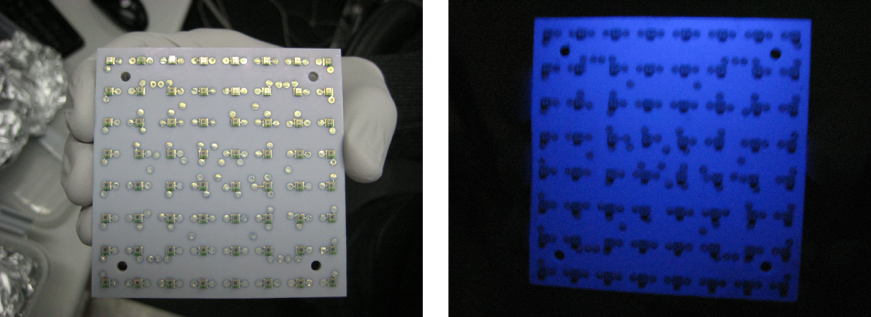
\includegraphics[scale=0.5]{img/DC.png}
	%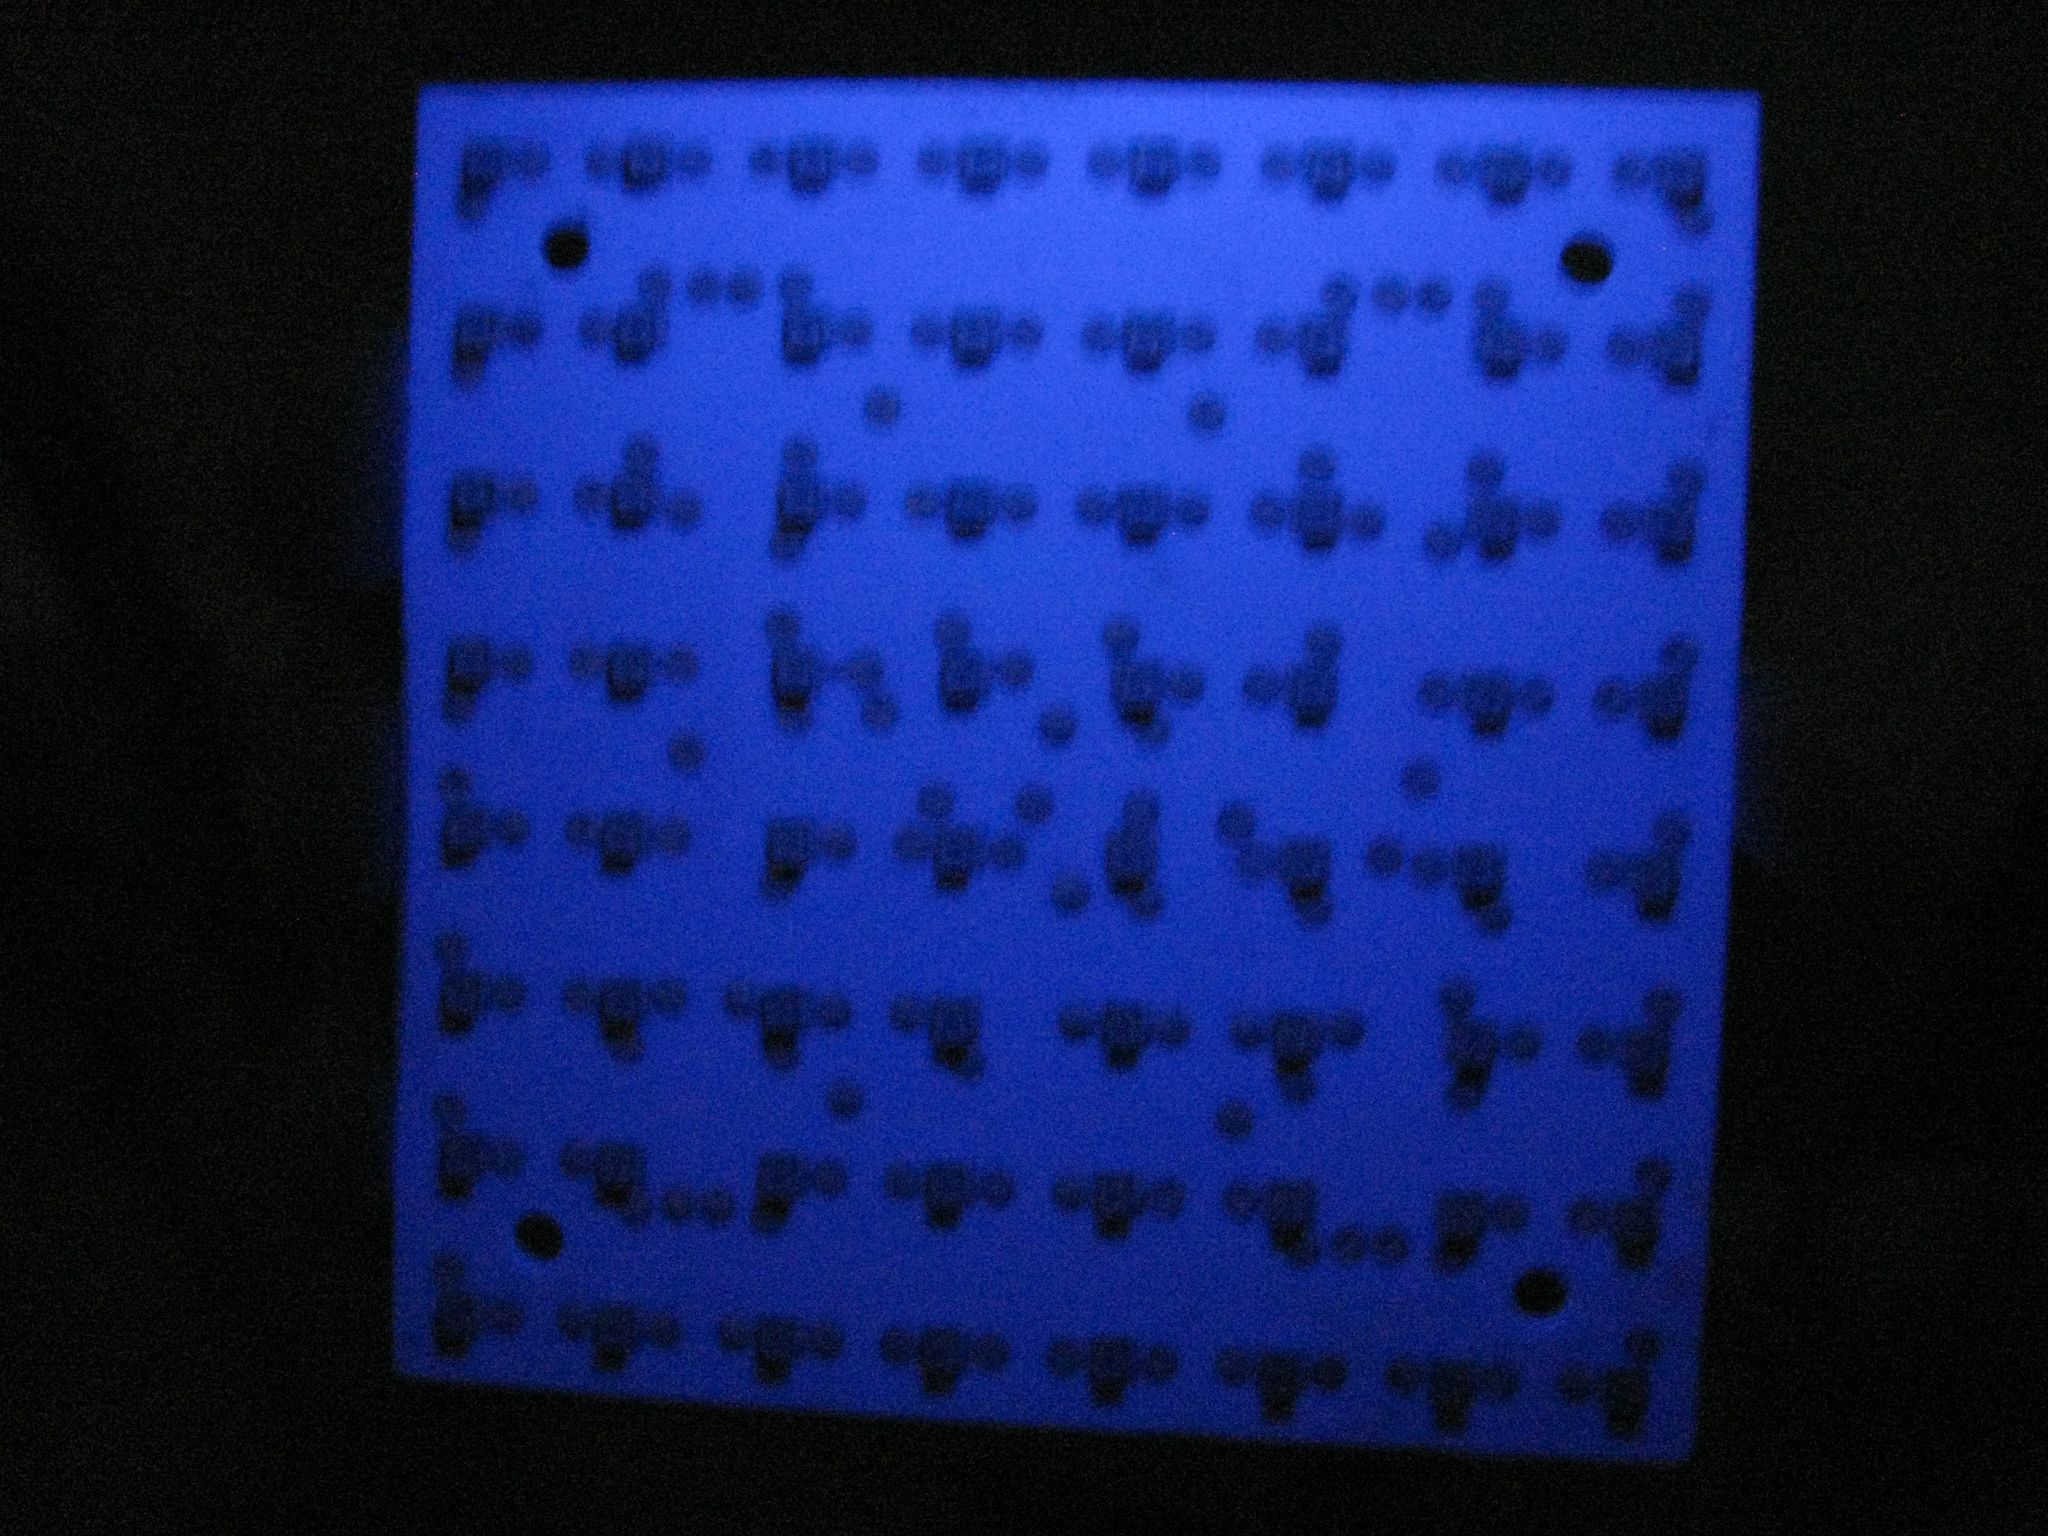
\includegraphics[scale=0.10]{img/DICE_Coated.jpg}
	\caption{\label{fig.DB} The top panel shows a DB made of Cuflon, developed for the NEXT-DEMO experiment. The DB is coated with TPB, which shifts the VUV light emitted by xenon (170 nm) to blue (420 nm). The right panel shows the response of a DB (emitting blue light) when illuminated with a UV lamp.  }
\end{figure}

Figure \ref{fig.DB} (top panel) ~shows a DB made of Cuflon, developed for the NEXT-DEMO detector. The DB is coated with TPB, which shifts the VUV light emitted by xenon (170 nm) to blue (420 nm). The bottom panel shows the response of a DB (emitting blue light) when illuminated with a UV lamp. The DBs of PETALO will have a similar design, except for the use of larger SiPMs (we are currently planning to use 6mm parts, available from several vendors).
Indeed the DBs for PETALO are easier to fabricate and much more economical than those developed for NEXT, since there are no radio purity restrictions, allowing the use of standard PCB materials such as FR4, which are forbidden in a radio pure application.

\subsection{The Liquid Xenon Scintillating Cell (LXSC):}

\label{sec.lxsc}

\begin{figure}[!htb]
	\centering
	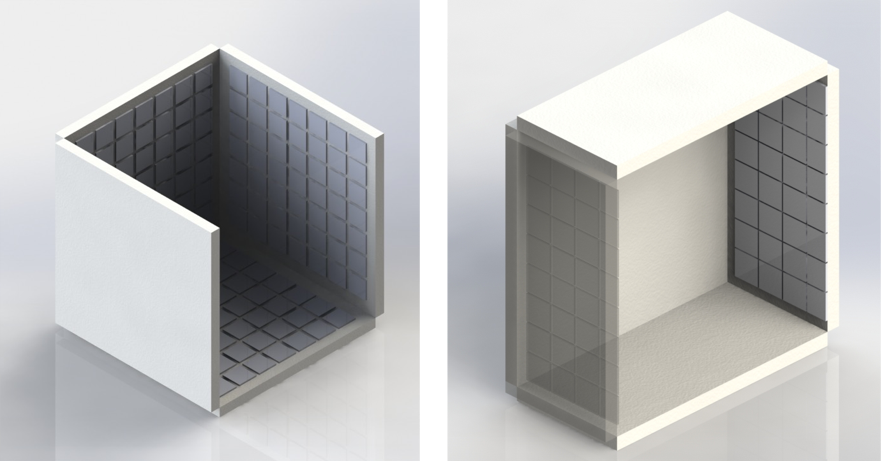
\includegraphics[scale=0.5]{img/lxsc2.png}
	%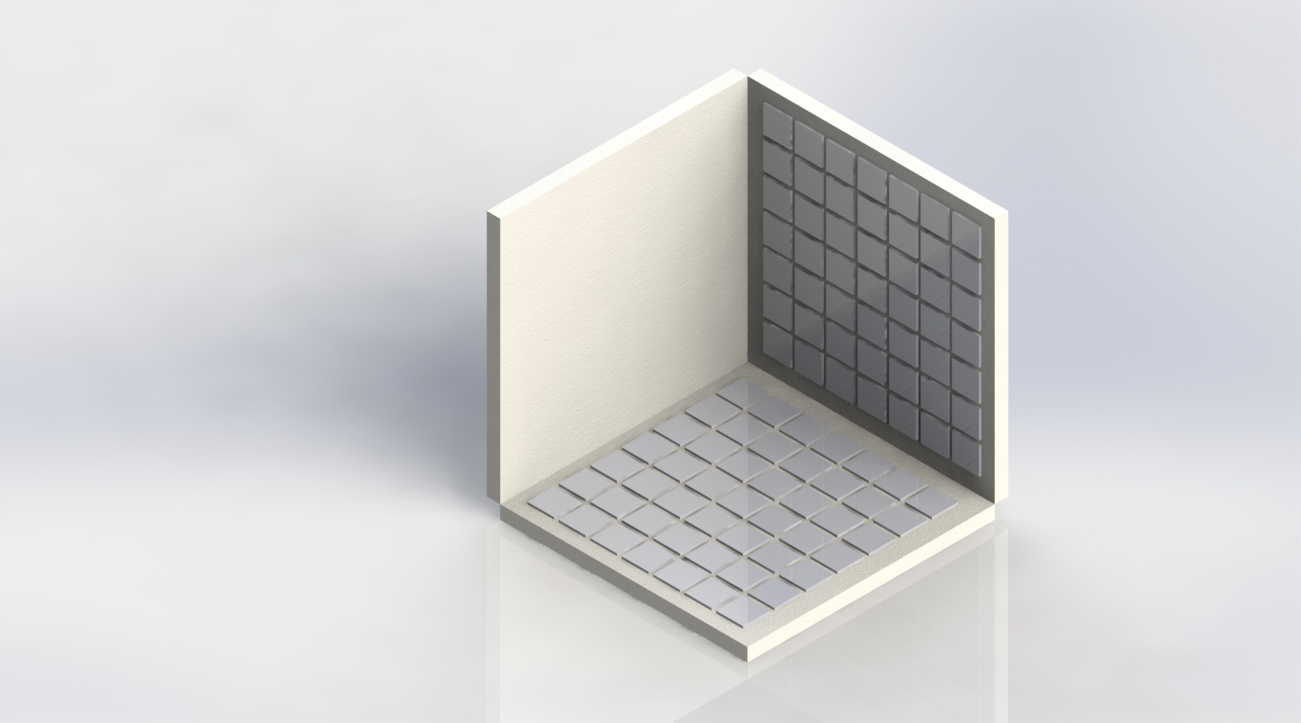
\includegraphics[scale=0.35]{img/box5open.jpg}
	\caption{\label{fig.box} The LXSC6 is a box of 
	$5\times 5 \times 5$~cm$^3$~with all its faces instrumented with SiPMs. In order to reduce costs, however, is feasible to instrument only two faces (LXSC2). The faces non instrumented are covered by reflecting teflon coated with TPB. }
\end{figure}

Figure \ref{fig.box}~shows a conceptual drawing of the keystone of the PETALO apparatus, the Liquid Xenon Scintillating Cell (LXSC). The cell is a box of $5\times 5 \times 5$~cm$^3$~ filled with liquid xenon and immersed in a cryostat. The cell transverse size (relative to the incoming beam) is optimised to minimise pileup and its longitudinal size is optimised so that most of the incoming 511 keV photons (80\%) interact in the volume. 

The best performance from the point of view of energy resolution is obtained when all the box faces are instrumented with SiPMs, as illustrated in the left panel of Figure \ref{fig.box}. We denote this configuration as LXSC6. On the other hand, the most economical configuration is obtained instrumenting only the entry and exit faces (relative to the beam direction). We call this configuration LXSC2. Other possible configurations instrument three faces (entry, exit and one of the lateral faces, LXSC3) or four faces (entry, exit and two opposite laterals, LXSC4). 
The faces non instrumented are covered by reflecting teflon coated with TPB. In section \ref{sec.mc} we show that an excellent performance can be obtained even with the sparse LXSC2 configuration. 

\section{Monte Carlo simulations of the LXSC}
\label{sec.mc}

\begin{figure}[!htb]
	\centering
	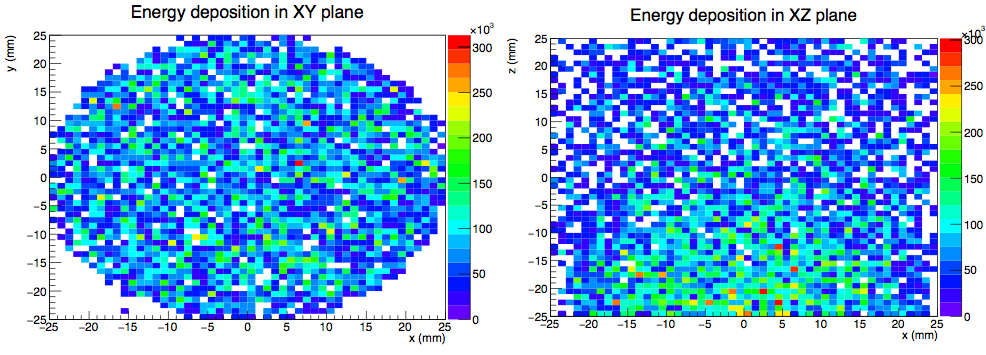
\includegraphics[scale=0.5]{img/gammas.png}
	\caption{\label{fig.gammas}  Left panel: (x,y) distribution of the gammas interacting in the LXSC. Right panel: (x,z) distribution, showing an accumulation of interactions in the first 3 cm.  }
\end{figure}

\begin{figure}[!htb]
	\centering
	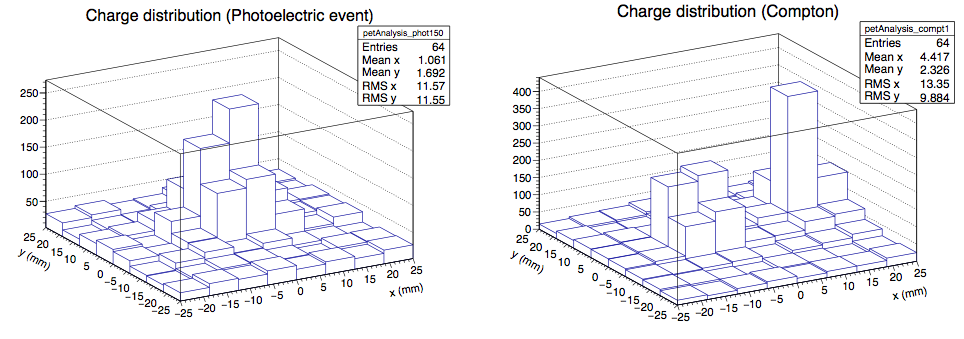
\includegraphics[scale=0.5]{img/Events.png}
	\caption{\label{fig.events}  Left panel: a photoelectric event in the LXSC, showing a single deposition cluster; right panel: A two-site Compton event.  }
\end{figure}

A full GEANT4 simulation has been carried out to study the performance of the LXSC. Photons of 511 keV enter the LXSC from outside (defining the ``entry face'') and interact in the cell (see Figure \ref{fig.gammas}), through photoelectric (around 20\% of the times, see Figure \ref{fig.events}, left panel) or Compton interactions (Figure \ref{fig.events}, right panel. About 60\% of the incoming gammas deposit their full energy in the LXSC. 

If $E$~ is the energy deposited by the ionising radiation (in this case 511 keV), the maximum scintillation yield of LXe is given as $E/W_{ph}$, where $W_{ph}$~ is the average energy required for the production of a single photon. The most probable value of $W_{ph}$~ in LXe  is\footnote{E. Aprile and T. Doke, Liquid Xenon Detectors for Particle Physics and Astrophysics, Rev. Mod. Phys. 82 (2010) 2053–2097, [arXiv:0910.4956].} is $13.8 \pm 0.9$~eV. Therefore, a maximum of 37,000 scintillation photons are produced when a 511 keV gamma interacts in the LXe. On the other hand, measurements carried out with electrons of 1 MeV result in a lower value of $W_{ph}^e = 21.6$\footnote{T. Doke, A. Hitachi, J. Kikuchi, K. Masuda, H. Okada and E. Shibamura: Jpn. J. Appl. Phys. 41 (2002) 1538.}. This lowest value is attributed to ionisation electrons that do not recombine, and would imply a yield of $\sim$ 24,000 scintillation photons for a 511 keV gammas. The results presented below are obtained assuming the maximum scintillation yield, but we also discuss the implications of a lowest scintillation yield in the energy and spacial resolution. 

\section{Energy resolution of the LXSC}

The VUV photons produced by the interactions of gammas in the LXSC are shifted to 420 nm by the TPB which coats the teflon panels and the SiPMs. The conversion efficiency, measured, among other authors by the NEXT collaboration is 80\%. The resulting blue photons are registered by the SiPMs, with high efficiency (the typical PDE of modern SiPMs for 420 nm exceeds 50\%. For this specific study we have simulated the 6 mm SENSL C-series sensor). 

While the fast decay time of scintillation (2 ns) allows for TOF applications (see below), the longer time associated with the recombination of electrons (45 ns) implies integration times of the order of 200-300 ns, similar to those used by LSO detectors. The dark current of the SiPMs and the electronic noise of the front-end electronics (in the case than an ASIC is used) is very low due to the cryogenic operation, and thus the resolution is dominated by photoelectron statistics. 

\begin{figure}[!htb]
	\centering
	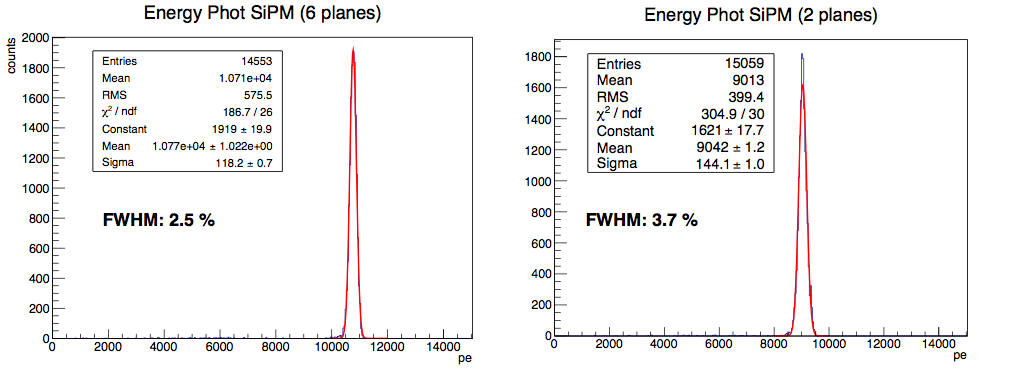
\includegraphics[scale=0.5]{img/energyResolution.png}
	\caption{\label{fig.energy}  Left panel: the intrinsic energy resolution of the LXSC6 is excellent (around 2.5\% FWHM) due to the high photoelectron statistics. Right panel: the most sparse configuration, LXSC2 records less light, but the resolution is still very good (3.7\% FWHM). }
\end{figure}

\begin{figure}[!htb]
	\centering
	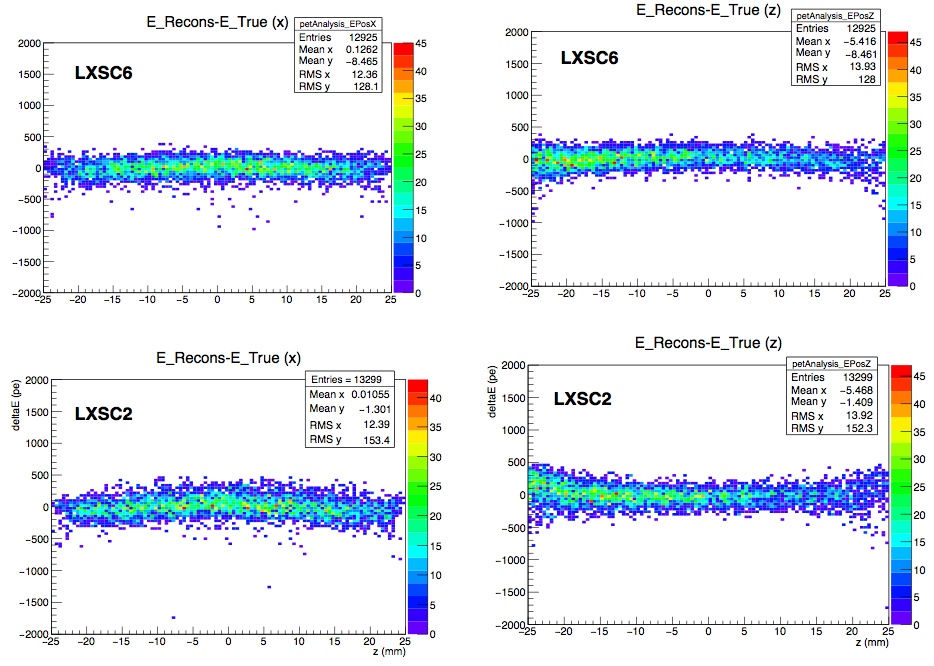
\includegraphics[scale=0.5]{img/EnergyPos.png}
	\caption{\label{fig.energyDep}  Top-left panel: the dependence of the energy with the transverse coordinate ($x$) in the LXSC6; top-right panel: the dependence of the energy with the longitudinal coordinate ($z$) in the LXSC6. The bottom-left and bottom-right panels show the dependence of the energy with the position for the LXSC2. Notice that the dependence of LXSC6 with position is very soft, while a stronger effect is observed in LXSC2, which is more sensitive to the solid angle covered by the interaction point.}
\end{figure}

Figure \ref{fig.energy} (left panel) shows the recorded number of photoelectrons in the LXSC6 corresponding to photoelectric interactions. The fit shows a resolution of 2.5\% FWHM, {\em much better} than the resolution obtained with conventional SSDs (for example, the best resolution obtained with test systems for LSO crystals is in the vicinity of 9 \% FWHM, while commercial PETs typically show a resolution of around 20 \% FWHM). The right panel shows the recorded number of photoelectrons in the LXSC2 corresponding to photoelectric interactions ($\sim$ 9000 P.E., to be compared with $\sim$ 12000 P.E. for the LXSC6). The  fit yields a resolution of 3.7\% FWHM. This is still very good, but it can be further improved by applying geometrical corrections.

The need for geometrical corrections is illustrated in Figure \ref{fig.energyDep}. The top panels show that the dependence of the energy with the longitudinal and transverse coordinate in the LXSC6 is very soft, and can be neglected for all practical purposes. This is indeed expected, as the LXSC6 is totally symmetric and solid angle effects are minimised. The effect is more visible, however, in the case of the LXSC2 (bottom panels), in particular in the transverse coordinate. Correcting this effect, a resolution of 3\% FWHM is achieved. 

If we assume the lowest $W_{ph}$~measured for electrons, the yield would be reduced by 65\% and the resolution of the LXSC2 would be around 3.5\% FWHM, much better than that of modern SSDs such as LSO. 

Notice that the small geometrical corrections found in the LXSC (even in the case of the LXSC2) are a crucial difference with the Waseda cell, where the geometrical corrections, due to the large size of the PMTs where very large and made, ultimately, the cell impractical as a detection device, since only the central part of the detector ($5 \times 5 \times 5$~mm$^3$) was useful. The second crucial difference that the LXSC registers much more light than the Waseda cell. This is due to the fact that all the faces are reflecting (the Waseda cell left one face open, resulting in large losses and fluctuations) and to the use of SiPMs, which have very large PDE ($\sim$ 50\% to be compared with the 5-20\% of the Waseda PMTs) right in the region (420 nm) where the light is shifted from TPB. 


%\begin{figure}[!htb]
%	\centering
%	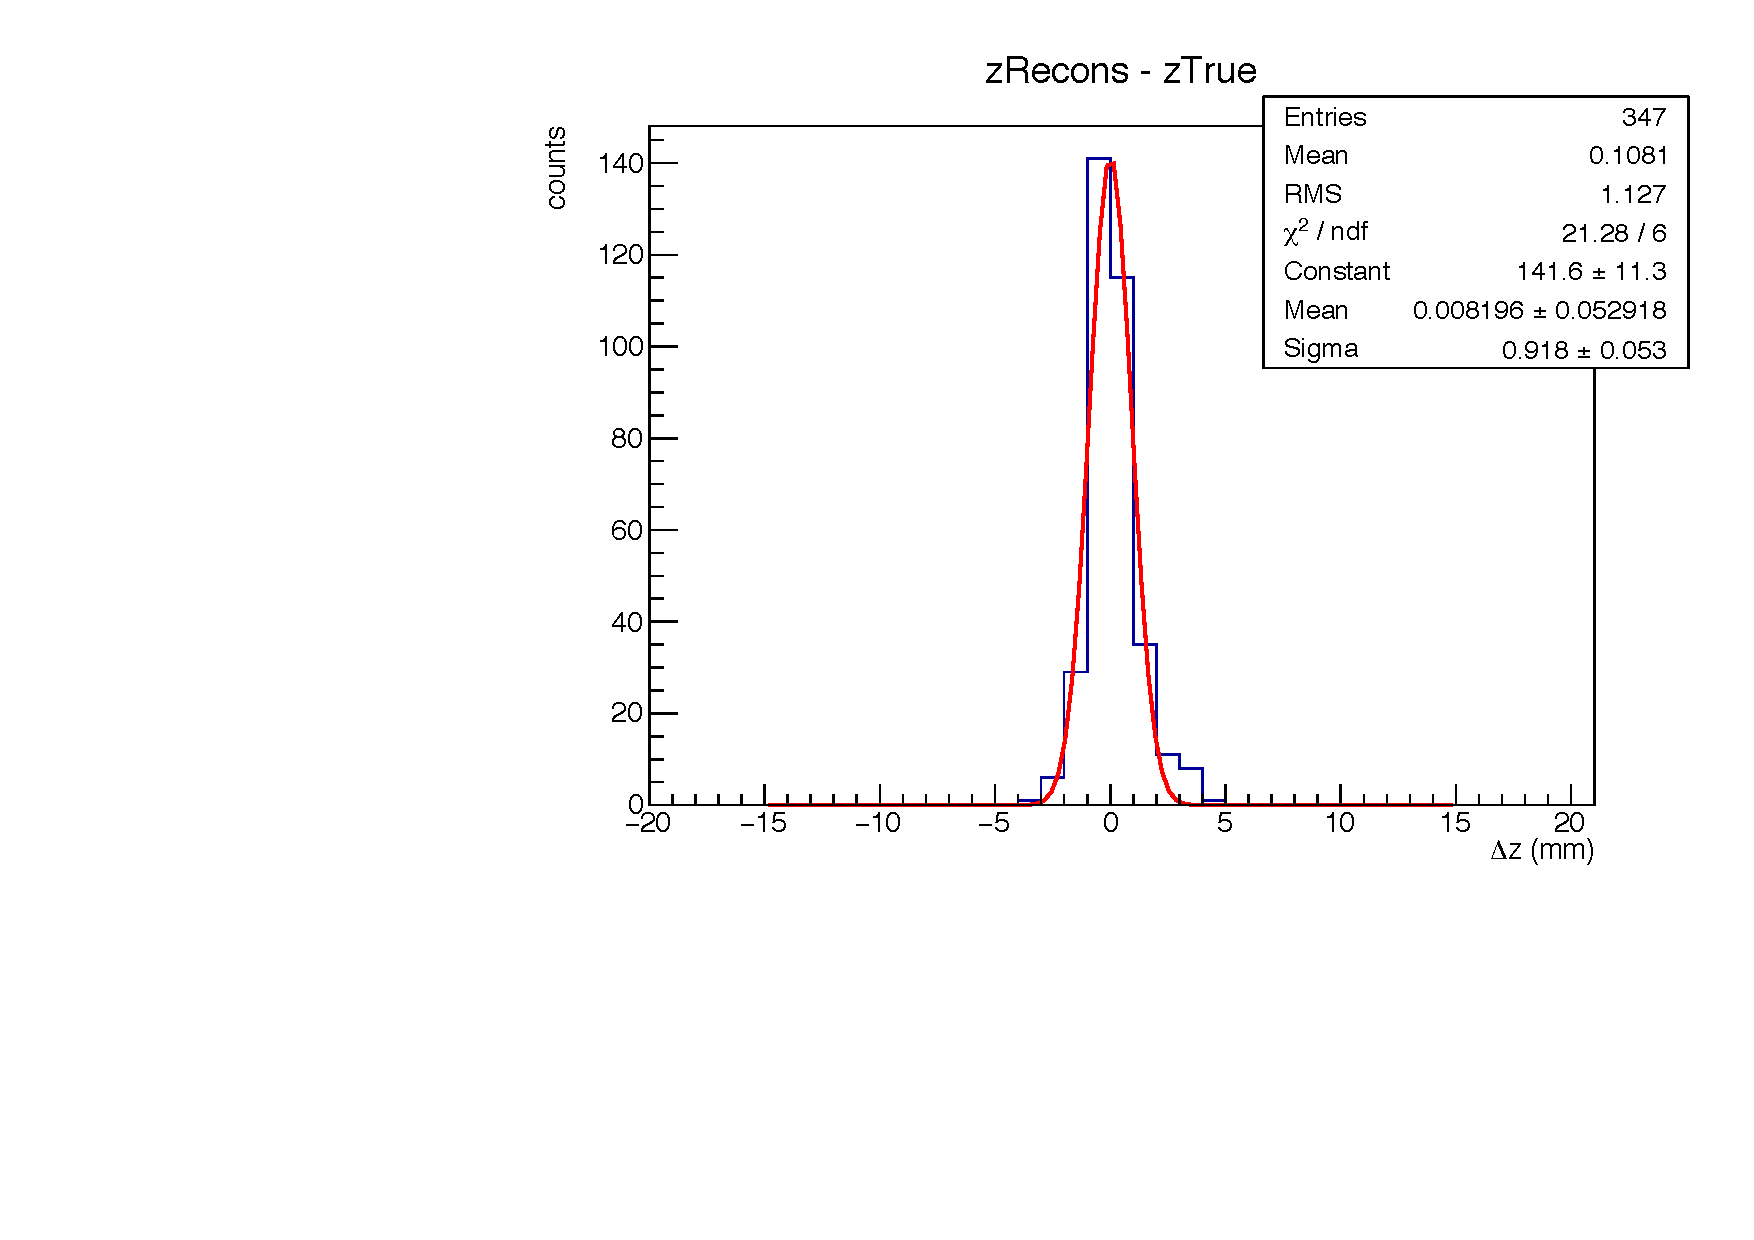
\includegraphics[scale=0.6]{img/zBest.pdf}
%	\caption{\label{fig.zbest}  Spacial resolution in the longitudinal coordinate ($z$). The transverse resolution is of the same order.  }
%\end{figure}

\section{Spatial resolution of the LXSC}

\begin{figure}[!htb]
	\centering
	\includegraphics[scale=0.4]{img/zEvents.png}
	\caption{\label{fig.ze}  Left panel: a photoelectric event interacting at $\sim$~2 cm from the entry face, leaving a distinct ``site signature'' (a cluster of SiPMs with charge higher than the rest. Right panel: the site signature (in the entry face) has all but disappeared when the gamma interacts near the exit face.}
\end{figure}

\begin{figure}[!htb]
	\centering
	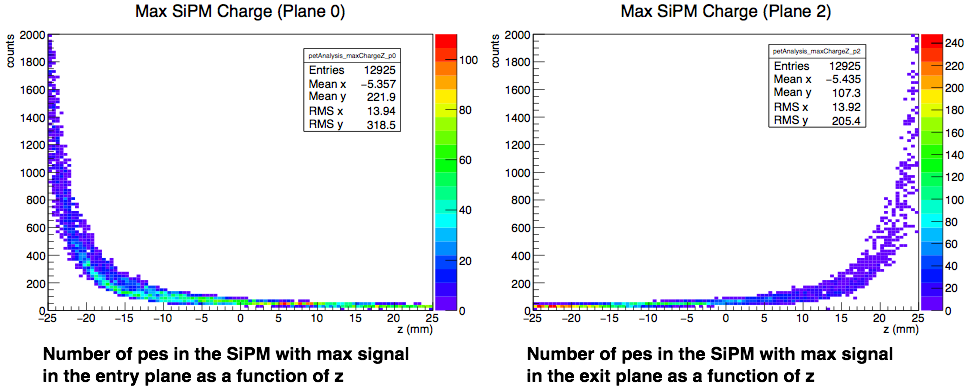
\includegraphics[scale=0.4]{img/SiPMMax.png}
	\caption{\label{fig.sipmm}  Left panel: Number of photoelectrons in the SiPMs registering the maximum signal as a function of the distance to the entry face. Number of photoelectrons in the SiPMs registering the maximum signal as a function of the distance to the exit face.}
\end{figure}

\begin{figure}[!htb]
	\centering
	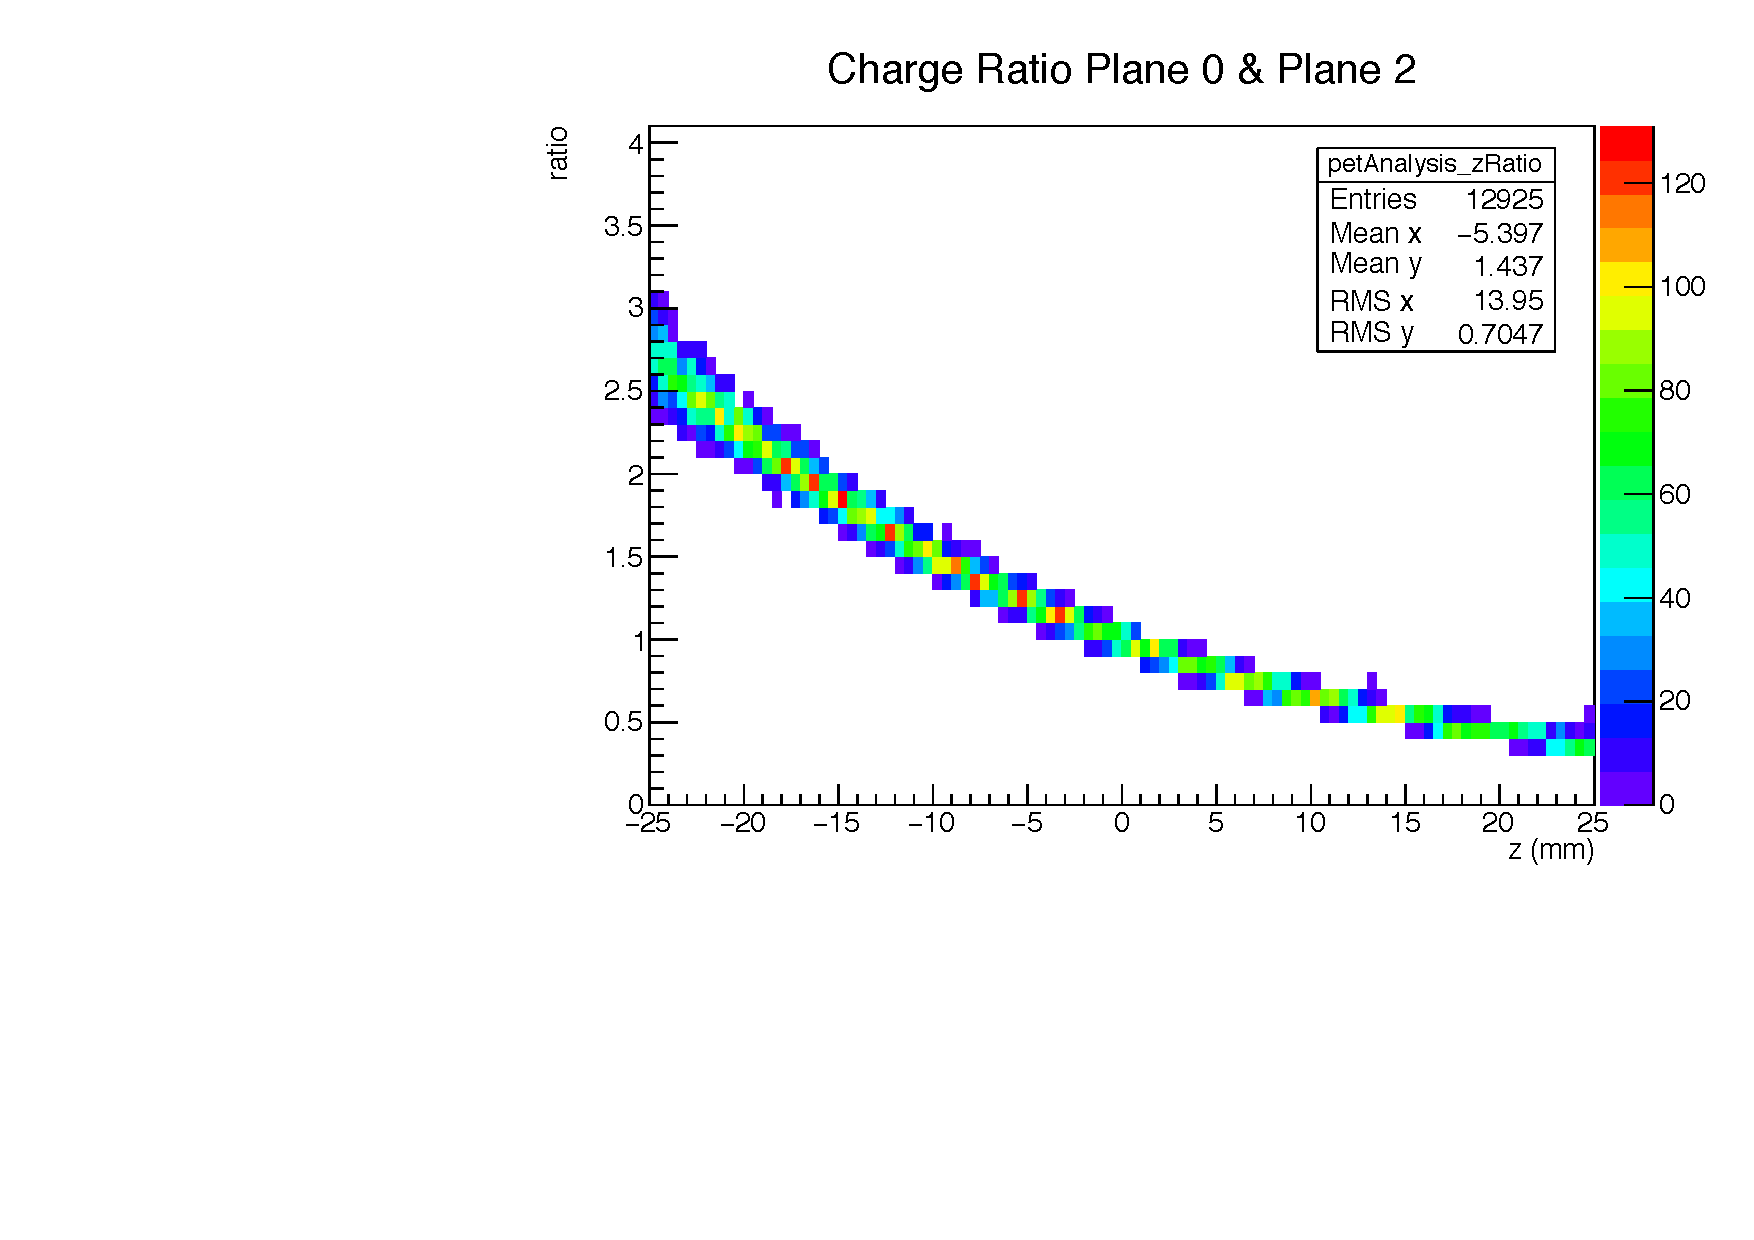
\includegraphics[scale=0.7]{img/z_ratio_totalCharge.pdf}
	\caption{\label{fig.zratio}  Ratio of the signal in the entry and the exit face (the signal in a face is defined as the sum of the signals of all its SiPMs) as a function of the longitudinal coordinate.}
\end{figure}

The simplest way to determine the point of interaction of an incoming photon, $(x,y,z)$~ is to use a barycentre algorithm. 
\[
\xi_r = \frac{\sum \xi_i N_i}{N}
\]
where $\xi_r$~stands for each one of the three coordinates ($x_r, y_r, z_r$), $N_i$~is the number of photoelectrons registered in each SiPM and $N=\sum N_i$. In the LXSC6 and LXSC4 configurations one can compute redundant measurements of $\xi_r$~for each coordinate. In the LXSC2 one can obtain ($x_r,y_r$) redundantly from the information found in the entry and exit faces and $z_r$~from the ratio of energy measured in the entry and the exit faces. This is illustrated by Figure \ref{fig.ze}, where the map of SiPMs in the entry face  is shown for gammas which interact: a) near the entry face; b) near the exit face. Clearly a baricenter algorithm using the information of the SiPMs in the entry face works well for gammas interacting in the first few cm of the cell (along the longitudinal coordinate), and may when the gammas are in the last two centimetres of the cell. However, when that happens, one can compute the baricenter using the exit face.  

This is illustrated quantitatively in Figure \ref{fig.sipmm}, which shows the number of photoelectrons in the SiPM registering the maximum signal (max signal sensor or MSS) as a function of the distance to the entry face (left panel) and the number of photoelectrons in the SiPMs registering the maximum signal as a function of the distance to the entry face (right panel). The signal of the MSS stays above 100 pes for the first (and the last) 2 cm of the cell, . In the central volume of about 1 cm, the position is determined by the combination of the signal found in both faces. 

Figure \ref{fig.zratio} shows the ratio of of the signal in the entry and the exit face (the signal in a face is defined as the sum of the signals of all its SiPMs) as a function of the longitudinal coordinate. The ratio measures the longitudinal coordinate.  

The space resolution obtained for the LXSC6 is better than 1 mm, which is of the same order of that attained by the best conventional SSDs equipped with SiPMs. The resolution in the LXSC2 is better than 2 mm in the transverse coordinates ($x,y$) and 1.5 mm in the longitudinal coordinates.  In addition, the resolution is achieved {\em in the three coordinates}, while conventional scintillators typically do not measure well the $z$~coordinate, a fact that introduces parallax errors. 


\section{PETALO as TOF-PET system}
\label{sec.tof}

%\begin{figure}[!htb]
%	\centering
%	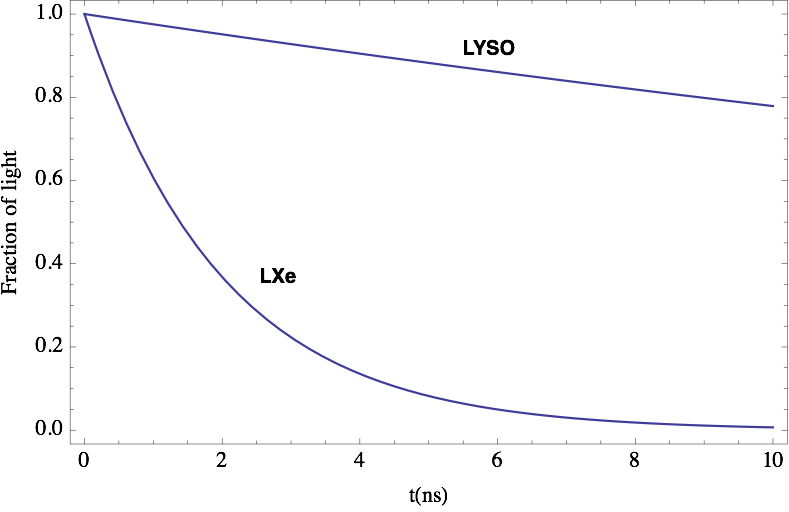
\includegraphics[scale=0.5]{img/TOF.png}
%	\caption{\label{fig.tof}  Decay time of LSO and LXe.  }
%\end{figure}

The quick decay time of xenon and the fast circuitry available in modern SiPMs offers an extraordinary potential for TOF applications. About 2.5\% of the photons are emitted in LXe in the first 50 ps after the interaction. The SiPM recording more signal in one event sees typically  2\% of the total photoelectrons (pes), and therefore it records 5 pes in the first 50 ps, enough to trigger a signal. For comparison, one nanosecond is needed in LSO to emit 2.5\% of the photons. Commercial TOF-PET systems based in LYSO (a proprietary version of LSO) have achieved a system time resolution of 600 ps. Since LXe features {\em both} higher light yield and much faster time response, a system resolution at the level or better than 200-250 ps appears possible. Thus PETALO could represent a break through in the field of PET-TOF. 

\section{Resolving Compton interactions}
\label{sec.comp}

Photoelectric interactions are a relatively small fraction of the total number of interactions in LXe (22\%) as well as in SSDs (for example, 33\% in LSO). The bulk of Compton interactions can result either in contained (when the scatter gamma produces a cascade that does not escape the detector) or non contained events. Non contained events do not deposit the full energy of the gamma in the detector and can be rejected. However, the large fraction of contained Compton events (60\% for the LXSC and larger for denser SSDs, such as LSO) introduce a significant distortion of the position in the case of conventional SSDs. Recall that conventional SSDs do not measure the $z$~(longitudinal) coordinate, introducing parallax errors. In addition, when a multiple-site Compton interaction occur in the detector, the transverse ($x,y$) coordinates are distorted, since the system only measures the average coordinate. 

Instead, in the LXSC, multiple-site hits are easily identified (the system measures true 3D points), and can be separated to a distance of the order of the detector pitch. This capability of separating photoelectric and Compton events in the LXSC can be further exploited in the case of 2-site Compton interactions. Resolving the position and the energy of both gammas with good resolution, allows the LXSC to operate as a {\em Compton Telescope}, taking advantage of Compton kinematics to further restrict the point of emission of the photons. 

%\section{Nuclear Magnetic Resonance compatibility}
%\label{sec.nmr}
%The LXSC  is built using non-magnetic materials, and unlike PMTs, SiPMs can operate in very high magnetic fields. Therefore PETALO can operate inside the very intense magnetic field generated by NMR devices. Furthermore, a NMS apparatus requires a large cryostat which can also accommodate the LXSC modules that make up PETALO. The technology offers, therefore, the possibility of building a fully NMR compatible device.  

\section{Conclusions}
\label{sec.conclu}

To summarise, PETALO offers the following advantages:

\begin{figure}[!htb]
	\centering
	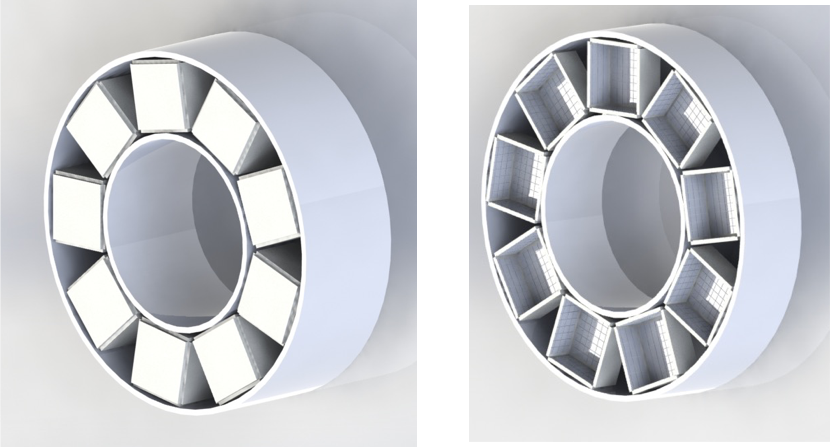
\includegraphics[scale=0.4]{img/SAP.png}
	\caption{\label{fig.smallPet} A conceptual drawing of a small animal PET, based in 9 LXSC. }
\end{figure}


\begin{enumerate}
\item Light yield higher than any conventional SSD.
\item Excellent intrinsic energy resolution (2.5 -- 3.5 \% FWHM depending on configuration of LXSC and of light yield). 
\item Excellent spatial resolution (1-2 mm in the three coordinates, minimising parallax error).
\item Capable of detecting multi-site Compton events. Thus suitable as Compton telescope.
\item Very fast time response, resulting in enhanced sensitivity (reduced number of random coincidences) and making it possible break-through TOF application. 
\item Fully NMR compatible. 
\item Competitive cost. The LXSC2 version of PETALO would cost today roughly half of the cost of the equivalent LSO unit. With the cost of SiPMs falling, the  cost of PET scanners will soon be fully dominated by the material of choice. Xenon is much cheaper than LSO and thus a large-scale apparatus (full body PET) is conceivable. 
\end{enumerate}

With respect to the pioneer work of the Waseda group, PETALO introduces the concept of the fully reflective LXSC, capable to detect the VUV light emitted by xenon with high efficiency and very small geometrical effects. The implementation of the LXSC using modern SIPMs may result in a break-through in PET technology. 


\acknowledgments

This work was supported by the European Research Council under the Advanced Grant 339787-NEXT and the Ministerio de Econom\'{i}a y Competitividad of Spain under Grants  FIS2014-53371-C4-1-R.

\bibliography{biblio}



\end{document}